\documentclass[aspectratio=169,11pt]{beamer}

\usepackage[T1]{fontenc}
\usepackage{lmodern}
\usepackage{amsmath,amssymb}
\usepackage{graphicx}
\usepackage{booktabs}

% figures live at the repo root
\graphicspath{{figs/}{../../}}

% ---------------------------------------------------------------- look
\definecolor{ink}{HTML}{1A1A19}
\definecolor{soft}{HTML}{52514E}
\definecolor{mblue}{HTML}{2A78D6}
\definecolor{morange}{HTML}{EB6834}
\definecolor{mgreen}{HTML}{199E70}
\definecolor{tint}{HTML}{F4F4F1}

\usetheme{default}
\usefonttheme{professionalfonts}
\setbeamertemplate{navigation symbols}{}
\setbeamercolor{normal text}{fg=ink,bg=white}
\setbeamercolor{structure}{fg=mblue}
\setbeamercolor{frametitle}{fg=ink}
\setbeamercolor{title}{fg=ink}
\setbeamercolor{subtitle}{fg=soft}
\setbeamercolor{author}{fg=soft}
\setbeamercolor{date}{fg=soft}
\setbeamercolor{footline}{fg=soft}
\setbeamercolor{block title}{fg=white,bg=mblue}
\setbeamercolor{block body}{fg=ink,bg=tint}
\setbeamerfont{frametitle}{series=\bfseries,size=\large}
\setbeamerfont{title}{series=\bfseries,size=\LARGE}
\setbeamertemplate{itemize items}[circle]
\setbeamertemplate{frametitle}{\vspace{0.6em}\insertframetitle\par\vspace{-0.35em}{\color{mblue}\rule{2.2cm}{1.2pt}}}
\setbeamertemplate{footline}{\hfill\usebeamercolor[fg]{footline}\scriptsize\insertframenumber\hspace{1.2em}\vspace{0.8em}}
\setlength{\leftmargini}{1.2em}

\newcommand{\hl}[1]{{\color{mblue}\textbf{#1}}}
\newcommand{\ho}[1]{{\color{morange}\textbf{#1}}}
\newcommand{\src}[1]{}
\newcommand{\fullfig}[2][0.98]{\begin{center}\includegraphics[width=#1\textwidth,height=0.64\textheight,keepaspectratio]{#2}\end{center}\vspace{-0.6em}}

\title{Monetary policy\\[0.2em]with and without time to build}
\date{October 2026}

\newcommand{\figslide}[1]{\begin{center}\includegraphics[width=\textwidth,height=0.82\textheight,keepaspectratio]{#1}\end{center}}

\begin{document}

\begin{frame}[plain]
  \vfill
  \titlepage
\end{frame}

% ==================================================================== MODEL
\begin{frame}{Model}
  Wage fixed: $W_t=\bar W$.

  \bigskip
  \textbf{Euler equation}
  \[
    \Xi_t\frac{C_t^{-\gamma}}{P_t}=\beta(1+i_t)\,\Xi_{t+1}\frac{C_{t+1}^{-\gamma}}{P_{t+1}}
  \]
  \textbf{Price index}
  \[
    P_t=\Biggl(\sum_j\Bigl[\frac{\bar W\prod_{s=t-\tau_j}^{t-1}(1+i_s)}{\zeta_j\,A_{t-\tau_j}}\Bigr]^{1-\sigma}\Biggr)^{\frac{1}{1-\sigma}}
  \]
\end{frame}

% --------------------------------------------------------------------
\begin{frame}{Planner's problem}
  \[
    \max_{\{i_t\}}\;U=\sum_t\beta^t\,\Xi_t\Bigl[\frac{C_t^{1-\gamma}}{1-\gamma}-\chi\frac{L_t^{1+\eta}}{1+\eta}\Bigr]
  \]
  \[
    \text{s.t. Euler, prices, price index, } C_t=Y_t;\qquad i_t\in[0,5\%]\text{ a month}
  \]
  \medskip
  \begin{itemize}\setlength{\itemsep}{0.6em}
    \item $L_t$: labour \hl{hired} at $t$ (for goods delivered at $t+\tau_j$)
    \item One period $=$ one month; rate free from the news date (or $t=0$) to $t=7$, then $\rho$
    \item Shocks: TFP $A_0=0.97$;\quad demand $\Xi_0=e^{-0.01}$
    \item $\gamma=\eta=2,\ \chi=1,\ \sigma=5,\ \kappa=0.938$;\ $\rho=0.33\%$ a month ($4\%$ a year); price $=$ marginal cost
  \end{itemize}
\end{frame}

% --------------------------------------------------------------------
\begin{frame}{Expected shocks, policy from $t=0$: TFP shock, no policy change}
  \figslide{ttb_expected0_tfp_peg.png}
\end{frame}

% --------------------------------------------------------------------
\begin{frame}{Expected shocks, policy from $t=0$: TFP shock}
  \figslide{ttb_expected0_tfp.png}
\end{frame}

% --------------------------------------------------------------------
\begin{frame}{Expected shocks, policy from $t=0$: demand shock, no policy change}
  \figslide{ttb_expected0_dem_peg.png}
\end{frame}

% --------------------------------------------------------------------
\begin{frame}{Expected shocks, policy from $t=0$: demand shock}
  \figslide{ttb_expected0_dem.png}
\end{frame}

% --------------------------------------------------------------------
\begin{frame}{Expected shocks, policy from $t=0$: where labour goes}
  \figslide{ttb_expected0_labour.png}
\end{frame}

% --------------------------------------------------------------------
\begin{frame}{Expected shocks, policy from $t=0$: firm profits}
  \figslide{ttb_expected0_profit.png}
\end{frame}

% --------------------------------------------------------------------
\begin{frame}{Expected shocks, policy from $t=0$: welfare gain from optimal policy}
  \figslide{ttb_policygain_expected0.png}
\end{frame}

% --------------------------------------------------------------------
\begin{frame}{Expected shocks, policy from the news: TFP shock, no policy change}
  \figslide{ttb_expected_pre_tfp_peg.png}
\end{frame}

% --------------------------------------------------------------------
\begin{frame}{Expected shocks, policy from the news: TFP shock}
  \figslide{ttb_expected_pre_tfp.png}
\end{frame}

% --------------------------------------------------------------------
\begin{frame}{Expected shocks, policy from the news: demand shock, no policy change}
  \figslide{ttb_expected_pre_dem_peg.png}
\end{frame}

% --------------------------------------------------------------------
\begin{frame}{Expected shocks, policy from the news: demand shock}
  \figslide{ttb_expected_pre_dem.png}
\end{frame}

% --------------------------------------------------------------------
\begin{frame}{Expected shocks, policy from the news: where labour goes}
  \figslide{ttb_expected_labour_pre.png}
\end{frame}

% --------------------------------------------------------------------
\begin{frame}{Expected shocks, policy from the news: firm profits}
  \figslide{ttb_expected_pre_profit.png}
\end{frame}

% --------------------------------------------------------------------
\begin{frame}{Expected shocks, policy from the news: welfare gain from optimal policy}
  \figslide{ttb_policygain_expected_news.png}
\end{frame}

% --------------------------------------------------------------------
\begin{frame}{Unexpected shocks, fixed wage: TFP shock, no policy change}
  \figslide{ttb_unexpected_tfp_peg.png}
\end{frame}

% --------------------------------------------------------------------
\begin{frame}{Unexpected shocks, fixed wage: TFP shock}
  \figslide{ttb_unexpected_tfp.png}
\end{frame}

% --------------------------------------------------------------------
\begin{frame}{Unexpected shocks, fixed wage: demand shock, no policy change}
  \figslide{ttb_unexpected_dem_peg.png}
\end{frame}

% --------------------------------------------------------------------
\begin{frame}{Unexpected shocks, fixed wage: demand shock}
  \figslide{ttb_unexpected_dem.png}
\end{frame}

% --------------------------------------------------------------------
\begin{frame}{Unexpected shocks, fixed wage: where labour goes}
  \figslide{ttb_unexpected_labour.png}
\end{frame}

% --------------------------------------------------------------------
\begin{frame}{Unexpected shocks, fixed wage: firm profits}
  \figslide{ttb_unexpected_profit.png}
\end{frame}

% --------------------------------------------------------------------
\begin{frame}{Unexpected shocks, fixed wage: welfare gain from optimal policy}
  \figslide{ttb_policygain_unexpected.png}
\end{frame}

% ==================================================================== NEWS 1 AHEAD
\begin{frame}{Shock announced 1 period ahead: TFP shock, no policy change}
  \figslide{ttb_news1_tfp_peg.png}
\end{frame}

% --------------------------------------------------------------------
\begin{frame}{Shock announced 1 period ahead: TFP shock}
  \figslide{ttb_news1_tfp.png}
\end{frame}

% --------------------------------------------------------------------
\begin{frame}{Shock announced 1 period ahead: demand shock, no policy change}
  \figslide{ttb_news1_dem_peg.png}
\end{frame}

% --------------------------------------------------------------------
\begin{frame}{Shock announced 1 period ahead: demand shock}
  \figslide{ttb_news1_dem.png}
\end{frame}

% --------------------------------------------------------------------
\begin{frame}{Shock announced 1 period ahead: where labour goes}
  \figslide{ttb_news1_labour.png}
\end{frame}

% --------------------------------------------------------------------
\begin{frame}{Shock announced 1 period ahead: firm profits}
  \figslide{ttb_news1_profit.png}
\end{frame}

% --------------------------------------------------------------------
\begin{frame}{Shock announced 1 period ahead: welfare gain from optimal policy}
  \figslide{ttb_news1_gain.png}
\end{frame}

% ==================================================================== NEWS 2 AHEAD
\begin{frame}{Shock announced 2 periods ahead: TFP shock, no policy change}
  \figslide{ttb_news2_tfp_peg.png}
\end{frame}

% --------------------------------------------------------------------
\begin{frame}{Shock announced 2 periods ahead: TFP shock}
  \figslide{ttb_news2_tfp.png}
\end{frame}

% --------------------------------------------------------------------
\begin{frame}{Shock announced 2 periods ahead: demand shock, no policy change}
  \figslide{ttb_news2_dem_peg.png}
\end{frame}

% --------------------------------------------------------------------
\begin{frame}{Shock announced 2 periods ahead: demand shock}
  \figslide{ttb_news2_dem.png}
\end{frame}

% --------------------------------------------------------------------
\begin{frame}{Shock announced 2 periods ahead: where labour goes}
  \figslide{ttb_news2_labour.png}
\end{frame}

% --------------------------------------------------------------------
\begin{frame}{Shock announced 2 periods ahead: firm profits}
  \figslide{ttb_news2_profit.png}
\end{frame}

% --------------------------------------------------------------------
\begin{frame}{Shock announced 2 periods ahead: welfare gain from optimal policy}
  \figslide{ttb_news2_gain.png}
\end{frame}

% ==================================================================== NEWS 3 AHEAD
\begin{frame}{Shock announced 3 periods ahead: TFP shock, no policy change}
  \figslide{ttb_news3_tfp_peg.png}
\end{frame}

% --------------------------------------------------------------------
\begin{frame}{Shock announced 3 periods ahead: TFP shock}
  \figslide{ttb_news3_tfp.png}
\end{frame}

% --------------------------------------------------------------------
\begin{frame}{Shock announced 3 periods ahead: demand shock, no policy change}
  \figslide{ttb_news3_dem_peg.png}
\end{frame}

% --------------------------------------------------------------------
\begin{frame}{Shock announced 3 periods ahead: demand shock}
  \figslide{ttb_news3_dem.png}
\end{frame}

% --------------------------------------------------------------------
\begin{frame}{Shock announced 3 periods ahead: where labour goes}
  \figslide{ttb_news3_labour.png}
\end{frame}

% --------------------------------------------------------------------
\begin{frame}{Shock announced 3 periods ahead: firm profits}
  \figslide{ttb_news3_profit.png}
\end{frame}

% --------------------------------------------------------------------
\begin{frame}{Shock announced 3 periods ahead: welfare gain from optimal policy}
  \figslide{ttb_news3_gain.png}
\end{frame}

% ==================================================================== NEWS 4 AHEAD
\begin{frame}{Shock announced 4 periods ahead: TFP shock, no policy change}
  \figslide{ttb_news4_tfp_peg.png}
\end{frame}

% --------------------------------------------------------------------
\begin{frame}{Shock announced 4 periods ahead: TFP shock}
  \figslide{ttb_news4_tfp.png}
\end{frame}

% --------------------------------------------------------------------
\begin{frame}{Shock announced 4 periods ahead: demand shock, no policy change}
  \figslide{ttb_news4_dem_peg.png}
\end{frame}

% --------------------------------------------------------------------
\begin{frame}{Shock announced 4 periods ahead: demand shock}
  \figslide{ttb_news4_dem.png}
\end{frame}

% --------------------------------------------------------------------
\begin{frame}{Shock announced 4 periods ahead: where labour goes}
  \figslide{ttb_news4_labour.png}
\end{frame}

% --------------------------------------------------------------------
\begin{frame}{Shock announced 4 periods ahead: firm profits}
  \figslide{ttb_news4_profit.png}
\end{frame}

% --------------------------------------------------------------------
\begin{frame}{Shock announced 4 periods ahead: welfare gain from optimal policy}
  \figslide{ttb_news4_gain.png}
\end{frame}

% ==================================================================== NEWS 5 AHEAD
\begin{frame}{Shock announced 5 periods ahead: TFP shock, no policy change}
  \figslide{ttb_news5_tfp_peg.png}
\end{frame}

% --------------------------------------------------------------------
\begin{frame}{Shock announced 5 periods ahead: TFP shock}
  \figslide{ttb_news5_tfp.png}
\end{frame}

% --------------------------------------------------------------------
\begin{frame}{Shock announced 5 periods ahead: demand shock, no policy change}
  \figslide{ttb_news5_dem_peg.png}
\end{frame}

% --------------------------------------------------------------------
\begin{frame}{Shock announced 5 periods ahead: demand shock}
  \figslide{ttb_news5_dem.png}
\end{frame}

% --------------------------------------------------------------------
\begin{frame}{Shock announced 5 periods ahead: where labour goes}
  \figslide{ttb_news5_labour.png}
\end{frame}

% --------------------------------------------------------------------
\begin{frame}{Shock announced 5 periods ahead: firm profits}
  \figslide{ttb_news5_profit.png}
\end{frame}

% --------------------------------------------------------------------
\begin{frame}{Shock announced 5 periods ahead: welfare gain from optimal policy}
  \figslide{ttb_news5_gain.png}
\end{frame}

% ==================================================================== NEWS 6 AHEAD
\begin{frame}{Shock announced 6 periods ahead: TFP shock, no policy change}
  \figslide{ttb_news6_tfp_peg.png}
\end{frame}

% --------------------------------------------------------------------
\begin{frame}{Shock announced 6 periods ahead: TFP shock}
  \figslide{ttb_news6_tfp.png}
\end{frame}

% --------------------------------------------------------------------
\begin{frame}{Shock announced 6 periods ahead: demand shock, no policy change}
  \figslide{ttb_news6_dem_peg.png}
\end{frame}

% --------------------------------------------------------------------
\begin{frame}{Shock announced 6 periods ahead: demand shock}
  \figslide{ttb_news6_dem.png}
\end{frame}

% --------------------------------------------------------------------
\begin{frame}{Shock announced 6 periods ahead: where labour goes}
  \figslide{ttb_news6_labour.png}
\end{frame}

% --------------------------------------------------------------------
\begin{frame}{Shock announced 6 periods ahead: firm profits}
  \figslide{ttb_news6_profit.png}
\end{frame}

% --------------------------------------------------------------------
\begin{frame}{Shock announced 6 periods ahead: welfare gain from optimal policy}
  \figslide{ttb_news6_gain.png}
\end{frame}

% ==================================================================== NEWS 7 AHEAD
\begin{frame}{Shock announced 7 periods ahead: TFP shock, no policy change}
  \figslide{ttb_news7_tfp_peg.png}
\end{frame}

% --------------------------------------------------------------------
\begin{frame}{Shock announced 7 periods ahead: TFP shock}
  \figslide{ttb_news7_tfp.png}
\end{frame}

% --------------------------------------------------------------------
\begin{frame}{Shock announced 7 periods ahead: demand shock, no policy change}
  \figslide{ttb_news7_dem_peg.png}
\end{frame}

% --------------------------------------------------------------------
\begin{frame}{Shock announced 7 periods ahead: demand shock}
  \figslide{ttb_news7_dem.png}
\end{frame}

% --------------------------------------------------------------------
\begin{frame}{Shock announced 7 periods ahead: where labour goes}
  \figslide{ttb_news7_labour.png}
\end{frame}

% --------------------------------------------------------------------
\begin{frame}{Shock announced 7 periods ahead: firm profits}
  \figslide{ttb_news7_profit.png}
\end{frame}

% --------------------------------------------------------------------
\begin{frame}{Shock announced 7 periods ahead: welfare gain from optimal policy}
  \figslide{ttb_news7_gain.png}
\end{frame}

% ==================================================================== NEWS 8 AHEAD
\begin{frame}{Shock announced 8 periods ahead: TFP shock, no policy change}
  \figslide{ttb_news8_tfp_peg.png}
\end{frame}

% --------------------------------------------------------------------
\begin{frame}{Shock announced 8 periods ahead: TFP shock}
  \figslide{ttb_news8_tfp.png}
\end{frame}

% --------------------------------------------------------------------
\begin{frame}{Shock announced 8 periods ahead: demand shock, no policy change}
  \figslide{ttb_news8_dem_peg.png}
\end{frame}

% --------------------------------------------------------------------
\begin{frame}{Shock announced 8 periods ahead: demand shock}
  \figslide{ttb_news8_dem.png}
\end{frame}

% --------------------------------------------------------------------
\begin{frame}{Shock announced 8 periods ahead: where labour goes}
  \figslide{ttb_news8_labour.png}
\end{frame}

% --------------------------------------------------------------------
\begin{frame}{Shock announced 8 periods ahead: firm profits}
  \figslide{ttb_news8_profit.png}
\end{frame}

% --------------------------------------------------------------------
\begin{frame}{Shock announced 8 periods ahead: welfare gain from optimal policy}
  \figslide{ttb_news8_gain.png}
\end{frame}

% ==================================================================== NEWS 9 AHEAD
\begin{frame}{Shock announced 9 periods ahead: TFP shock, no policy change}
  \figslide{ttb_news9_tfp_peg.png}
\end{frame}

% --------------------------------------------------------------------
\begin{frame}{Shock announced 9 periods ahead: TFP shock}
  \figslide{ttb_news9_tfp.png}
\end{frame}

% --------------------------------------------------------------------
\begin{frame}{Shock announced 9 periods ahead: demand shock, no policy change}
  \figslide{ttb_news9_dem_peg.png}
\end{frame}

% --------------------------------------------------------------------
\begin{frame}{Shock announced 9 periods ahead: demand shock}
  \figslide{ttb_news9_dem.png}
\end{frame}

% --------------------------------------------------------------------
\begin{frame}{Shock announced 9 periods ahead: where labour goes}
  \figslide{ttb_news9_labour.png}
\end{frame}

% --------------------------------------------------------------------
\begin{frame}{Shock announced 9 periods ahead: firm profits}
  \figslide{ttb_news9_profit.png}
\end{frame}

% --------------------------------------------------------------------
\begin{frame}{Shock announced 9 periods ahead: welfare gain from optimal policy}
  \figslide{ttb_news9_gain.png}
\end{frame}

% ==================================================================== NEWS 10 AHEAD
\begin{frame}{Shock announced 10 periods ahead: TFP shock, no policy change}
  \figslide{ttb_news10_tfp_peg.png}
\end{frame}

% --------------------------------------------------------------------
\begin{frame}{Shock announced 10 periods ahead: TFP shock}
  \figslide{ttb_news10_tfp.png}
\end{frame}

% --------------------------------------------------------------------
\begin{frame}{Shock announced 10 periods ahead: demand shock, no policy change}
  \figslide{ttb_news10_dem_peg.png}
\end{frame}

% --------------------------------------------------------------------
\begin{frame}{Shock announced 10 periods ahead: demand shock}
  \figslide{ttb_news10_dem.png}
\end{frame}

% --------------------------------------------------------------------
\begin{frame}{Shock announced 10 periods ahead: where labour goes}
  \figslide{ttb_news10_labour.png}
\end{frame}

% --------------------------------------------------------------------
\begin{frame}{Shock announced 10 periods ahead: firm profits}
  \figslide{ttb_news10_profit.png}
\end{frame}

% --------------------------------------------------------------------
\begin{frame}{Shock announced 10 periods ahead: welfare gain from optimal policy}
  \figslide{ttb_news10_gain.png}
\end{frame}

% ==================================================================== NEWS 11 AHEAD
\begin{frame}{Shock announced 11 periods ahead: TFP shock, no policy change}
  \figslide{ttb_news11_tfp_peg.png}
\end{frame}

% --------------------------------------------------------------------
\begin{frame}{Shock announced 11 periods ahead: TFP shock}
  \figslide{ttb_news11_tfp.png}
\end{frame}

% --------------------------------------------------------------------
\begin{frame}{Shock announced 11 periods ahead: demand shock, no policy change}
  \figslide{ttb_news11_dem_peg.png}
\end{frame}

% --------------------------------------------------------------------
\begin{frame}{Shock announced 11 periods ahead: demand shock}
  \figslide{ttb_news11_dem.png}
\end{frame}

% --------------------------------------------------------------------
\begin{frame}{Shock announced 11 periods ahead: where labour goes}
  \figslide{ttb_news11_labour.png}
\end{frame}

% --------------------------------------------------------------------
\begin{frame}{Shock announced 11 periods ahead: firm profits}
  \figslide{ttb_news11_profit.png}
\end{frame}

% --------------------------------------------------------------------
\begin{frame}{Shock announced 11 periods ahead: welfare gain from optimal policy}
  \figslide{ttb_news11_gain.png}
\end{frame}

% ==================================================================== NEWS 12 AHEAD
\begin{frame}{Shock announced 12 periods ahead: TFP shock, no policy change}
  \figslide{ttb_news12_tfp_peg.png}
\end{frame}

% --------------------------------------------------------------------
\begin{frame}{Shock announced 12 periods ahead: TFP shock}
  \figslide{ttb_news12_tfp.png}
\end{frame}

% --------------------------------------------------------------------
\begin{frame}{Shock announced 12 periods ahead: demand shock, no policy change}
  \figslide{ttb_news12_dem_peg.png}
\end{frame}

% --------------------------------------------------------------------
\begin{frame}{Shock announced 12 periods ahead: demand shock}
  \figslide{ttb_news12_dem.png}
\end{frame}

% --------------------------------------------------------------------
\begin{frame}{Shock announced 12 periods ahead: where labour goes}
  \figslide{ttb_news12_labour.png}
\end{frame}

% --------------------------------------------------------------------
\begin{frame}{Shock announced 12 periods ahead: firm profits}
  \figslide{ttb_news12_profit.png}
\end{frame}

% --------------------------------------------------------------------
\begin{frame}{Shock announced 12 periods ahead: welfare gain from optimal policy}
  \figslide{ttb_news12_gain.png}
\end{frame}

% ==================================================================== NEWS HORIZON SUMMARY
\begin{frame}{News horizons: summary}
  \figslide{ttb_horizon_summary.png}
\end{frame}

% --------------------------------------------------------------------
\begin{frame}{News horizons: welfare gain from optimal policy}
  \vspace{-0.6em}
  \centering\footnotesize\renewcommand{\arraystretch}{0.92}
  \begin{tabular}{lrr}
    \toprule
    $k$ & TFP & demand ($\times10^{-3}$)\\
    \midrule
    0 (unexp.) & 0.123 & 2.18\\
    1 & 0.371 & 2.68\\
    2 & 0.394 & 2.71\\
    3 & 0.392 & 2.45\\
    4 & 0.388 & 2.35\\
    5 & 0.387 & 2.34\\
    6 & 0.385 & 2.35\\
    7 & 0.385 & 2.35\\
    8 & 0.385 & 2.36\\
    9 & 0.384 & 2.36\\
    10 & 0.384 & 2.36\\
    11 & 0.384 & 2.36\\
    12 & 0.384 & 2.36\\
    13 & 0.384 & 2.36\\
    \bottomrule
  \end{tabular}

  \smallskip
  \raggedright\scriptsize
  Time to build.\quad Gain $=$ optimal $-$ peg, \% of one month's SS consumption, valued at $t=-13$.\quad No time to build: 0.011 / 0.008 (TFP), 3.65 (demand).
\end{frame}

% --------------------------------------------------------------------
\begin{frame}{News horizons: planner informed, firms and households not}
  \figslide{ttb_horizon_summary_planner.png}
\end{frame}

% --------------------------------------------------------------------
\begin{frame}{Who should know? Household welfare under the optimal rate}
  \centering\footnotesize
  \begin{tabular}{lrrrrrr}
    \toprule
    & \multicolumn{3}{c}{TFP} & \multicolumn{3}{c}{demand ($\times10^{-3}$)}\\
    \cmidrule(lr){2-4}\cmidrule(lr){5-7}
    $k$ & planner only & everyone & difference & planner only & everyone & difference\\
    \midrule
    0 (no warning) & 0 & 0 & $0$ & 0 & 0 & $0$\\
    1 & $+0.006$ & $-0.029$ & \textbf{+0.035} & $-0.11$ & $+1.13$ & \textbf{$-$1.24}\\
    2 & $+0.008$ & $-0.041$ & \textbf{+0.048} & $-0.04$ & $+1.66$ & \textbf{$-$1.70}\\
    3 & $+0.009$ & $-0.047$ & \textbf{+0.055} & $+0.01$ & $+1.85$ & \textbf{$-$1.84}\\
    5 & $+0.009$ & $-0.051$ & \textbf{+0.060} & $+0.05$ & $+1.99$ & \textbf{$-$1.94}\\
    8 & $+0.009$ & $-0.053$ & \textbf{+0.062} & $+0.05$ & $+2.02$ & \textbf{$-$1.97}\\
    13 & $+0.009$ & $-0.054$ & \textbf{+0.063} & $+0.05$ & $+2.02$ & \textbf{$-$1.97}\\
    \bottomrule
  \end{tabular}

  \bigskip
  \raggedright\scriptsize
  Time to build.\quad Utility under the optimal rate relative to no warning, \% of one month's SS consumption, valued at $t=-13$.\quad Difference $=$ planner only $-$ everyone informed.
\end{frame}


% ==================================================================== APPENDIX
\begin{frame}{Appendix: shock figures}
  \begin{itemize}\setlength{\itemsep}{0.8em}
    \item $c_t,\ n_t$: $100\log(X_t/X^{ss})$;\quad $n_t$ = labour \hl{hired} at $t$
    \item $\pi_t=100\,(\log P_t-\log P_{t-1})$ (\% a month),\quad $P_{-1}=P^{ss}$;\quad $i_t$ annualised
    \item Both: exact Euler, $W_t=W^{ss}$, labour dated at hiring in $U$
    \item Expected: shock announced at $t=-13$ (months);\quad unexpected: news at $t=0$
    \item Optimal: $\max U$ over $i_t$ up to $t=7$, then $\rho$;\quad $i_t\in[0,5\%]$\\
          free from $t=0$, or from the news date ($t=-13$, expected only)
    \item No time to build: same firms, $\tau_j\equiv0$
  \end{itemize}
\end{frame}

% --------------------------------------------------------------------
\begin{frame}{Appendix: where labour goes}
  Labour hired at $t$ by firm $j$, for its delivery at $t+\tau_j$:
  \[
    l_{j,t}=\frac{y_{j,t+\tau_j}}{\zeta_j A_t}
  \]
  Bar for lag group $g\in\{0,1,2,3,4,5^+\}$:
  \[
    b_{g,t}=100\,\frac{\sum_{j\in g}l_{j,t}-\sum_{j\in g}l_j^{ss}}{L^{ss}},\qquad
    L^{ss}=\sum_j l_j^{ss},\qquad
    \sum_g b_{g,t}=100\,\frac{L_t-L^{ss}}{L^{ss}}\approx n_t
  \]
  \centering
  \begin{tabular}{lrrrrrr}
    \toprule
    $\tau$ & 0 & 1 & 2 & 3 & 4 & 5+\\
    \midrule
    SS share of $L$, \% & 0.7 & 17.4 & 42.7 & 22.2 & 12.7 & 4.3\\
    \bottomrule
  \end{tabular}

  \medskip
  \raggedright
  $b_{g,t}$ = (group's own \% change) $\times$ (its share). Time to build only.
\end{frame}

% --------------------------------------------------------------------
\begin{frame}{Appendix: loss vs flexible wage, expected, policy from $t=0$}
  \begin{center}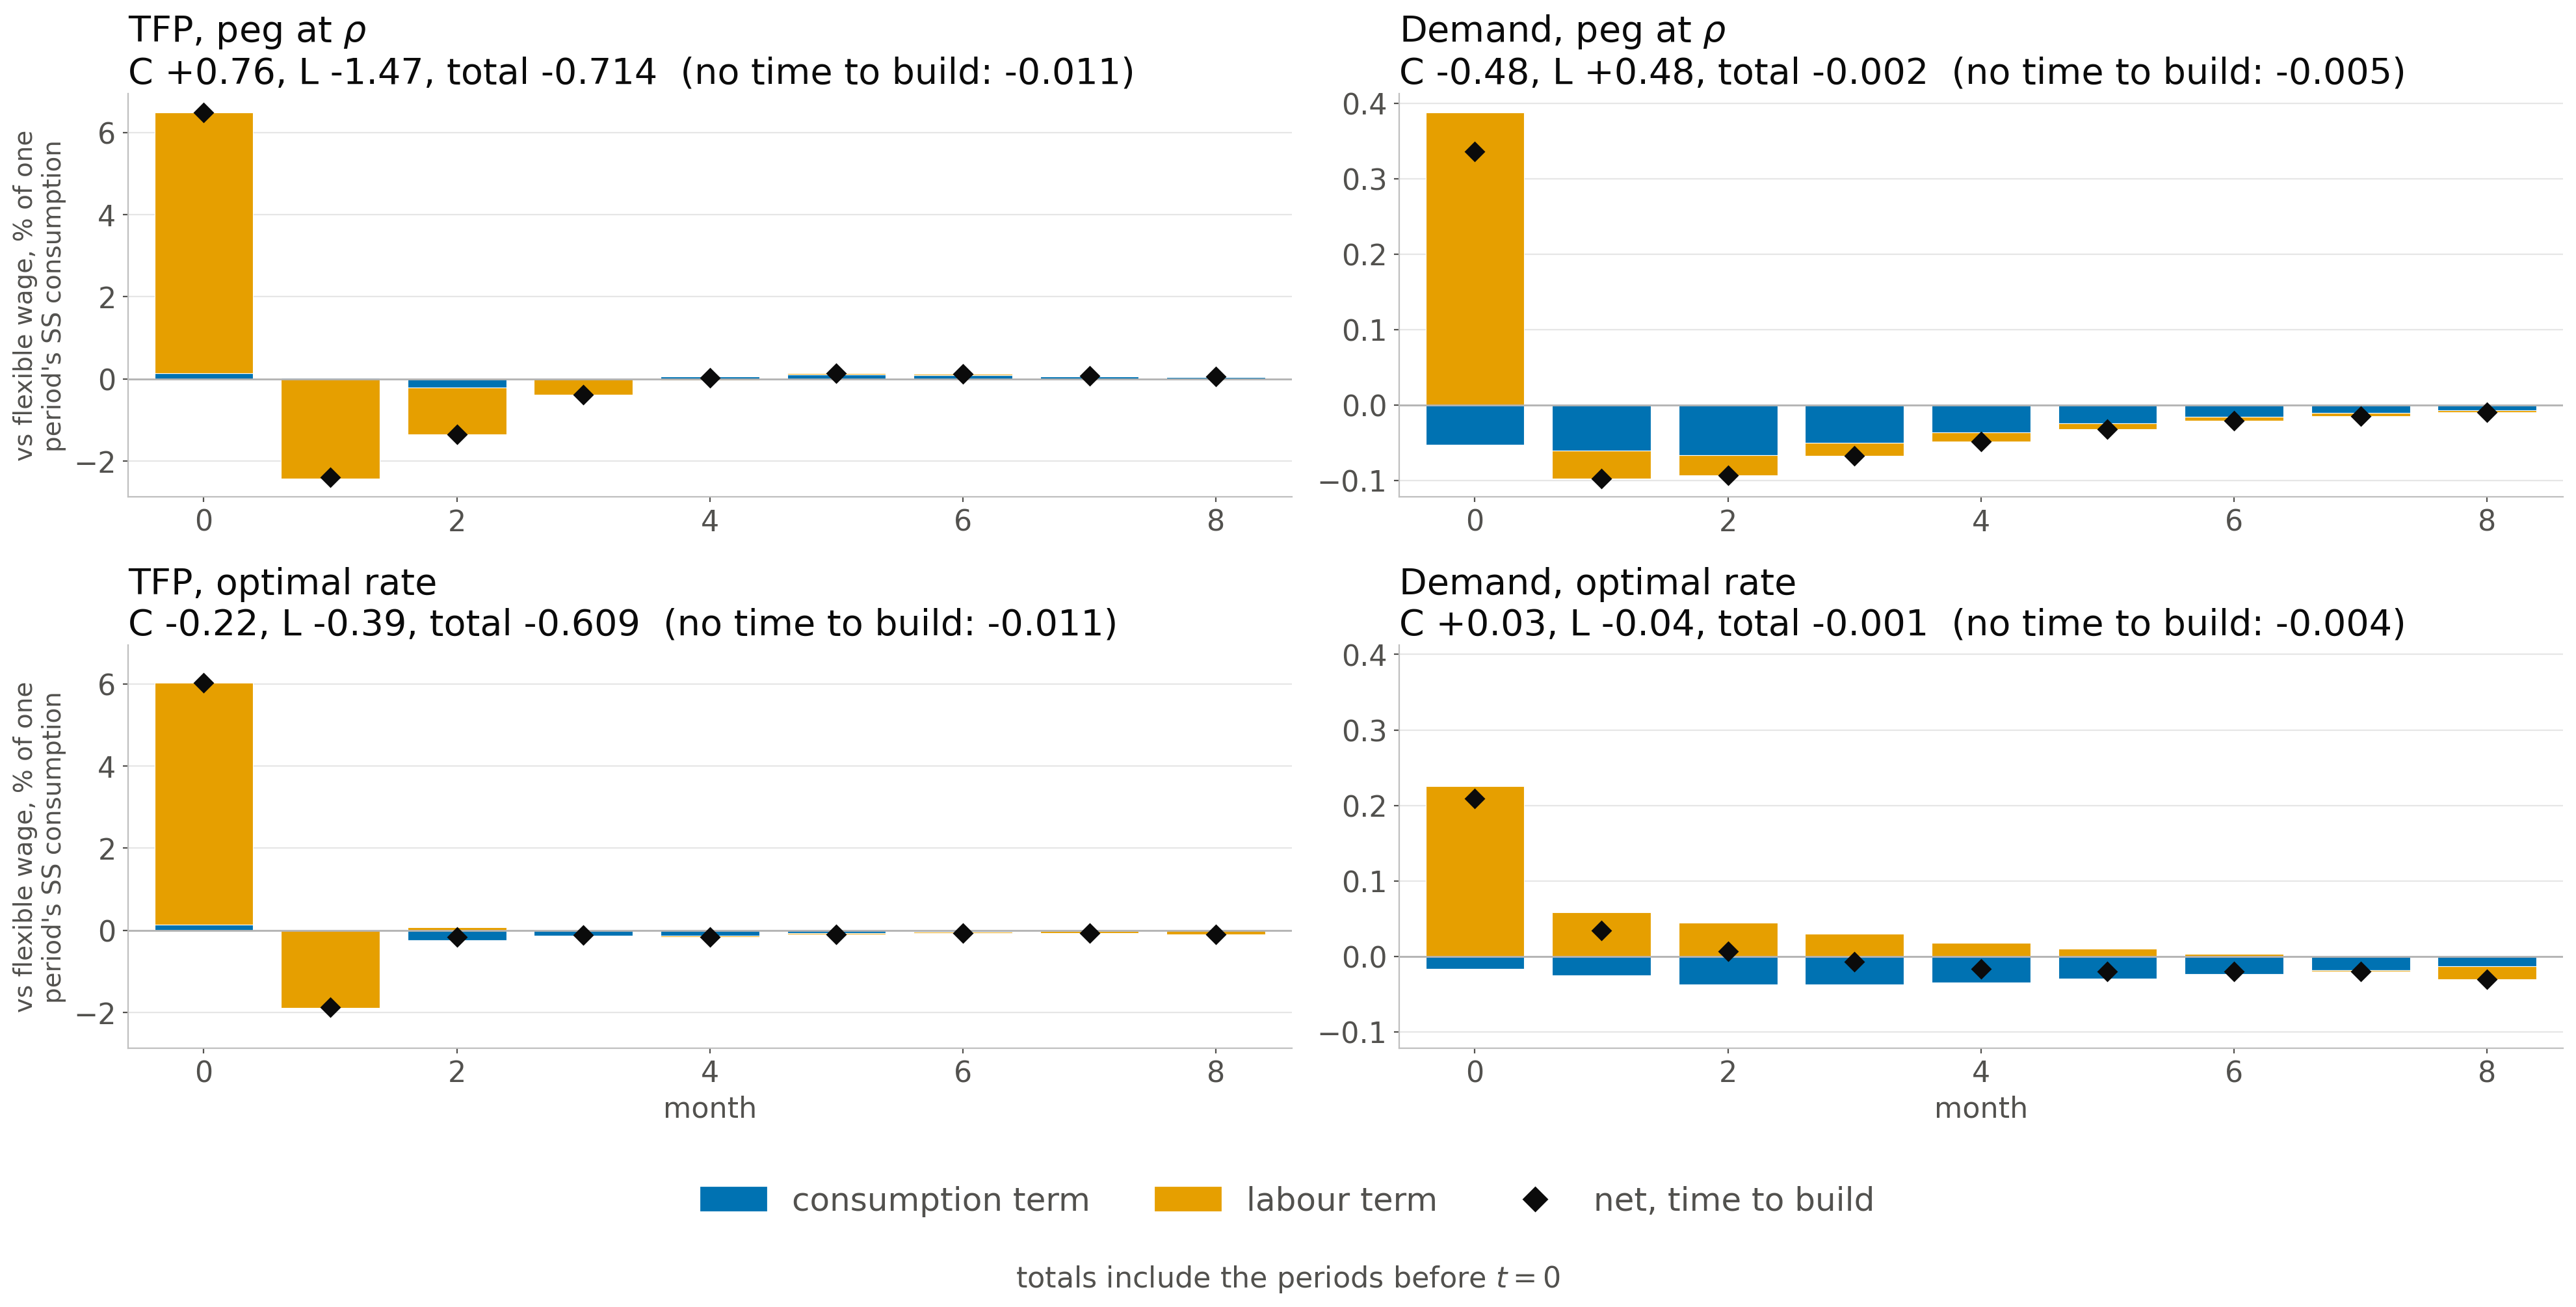
\includegraphics[width=\textwidth,height=0.76\textheight,keepaspectratio]{ttb_loss_expected0.png}\end{center}
\end{frame}

% --------------------------------------------------------------------
\begin{frame}{Appendix: loss vs flexible wage, expected, policy from news}
  \begin{center}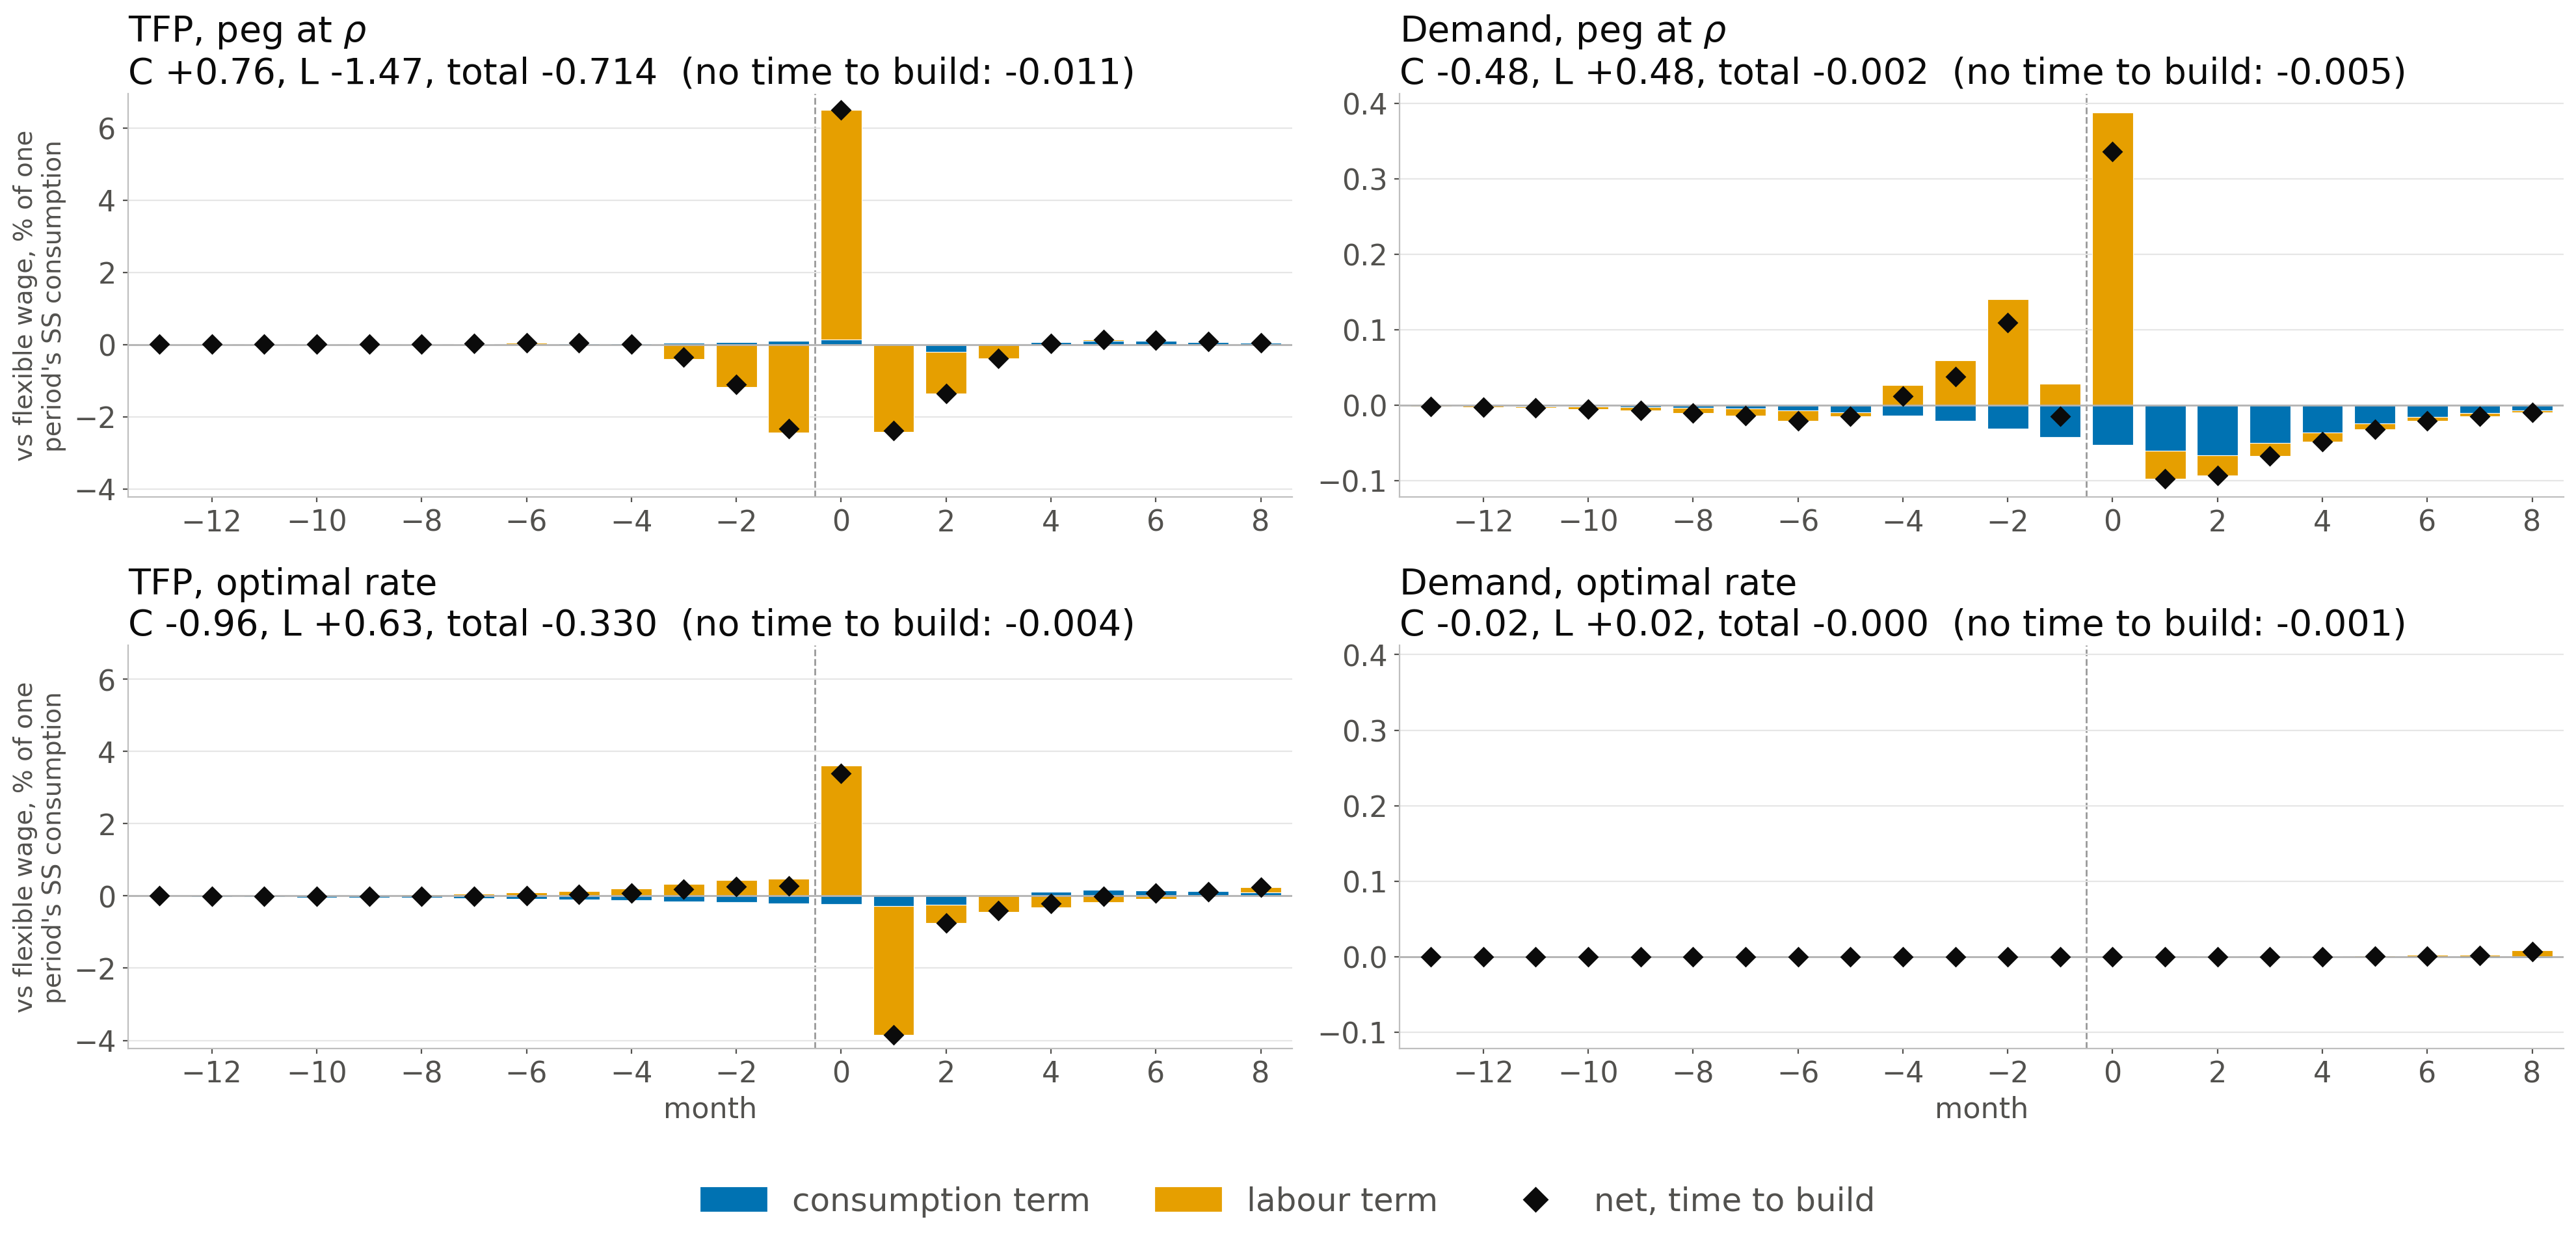
\includegraphics[width=\textwidth,height=0.76\textheight,keepaspectratio]{ttb_loss_expected_news.png}\end{center}
\end{frame}

% --------------------------------------------------------------------
\begin{frame}{Appendix: loss vs flexible wage, unexpected}
  \begin{center}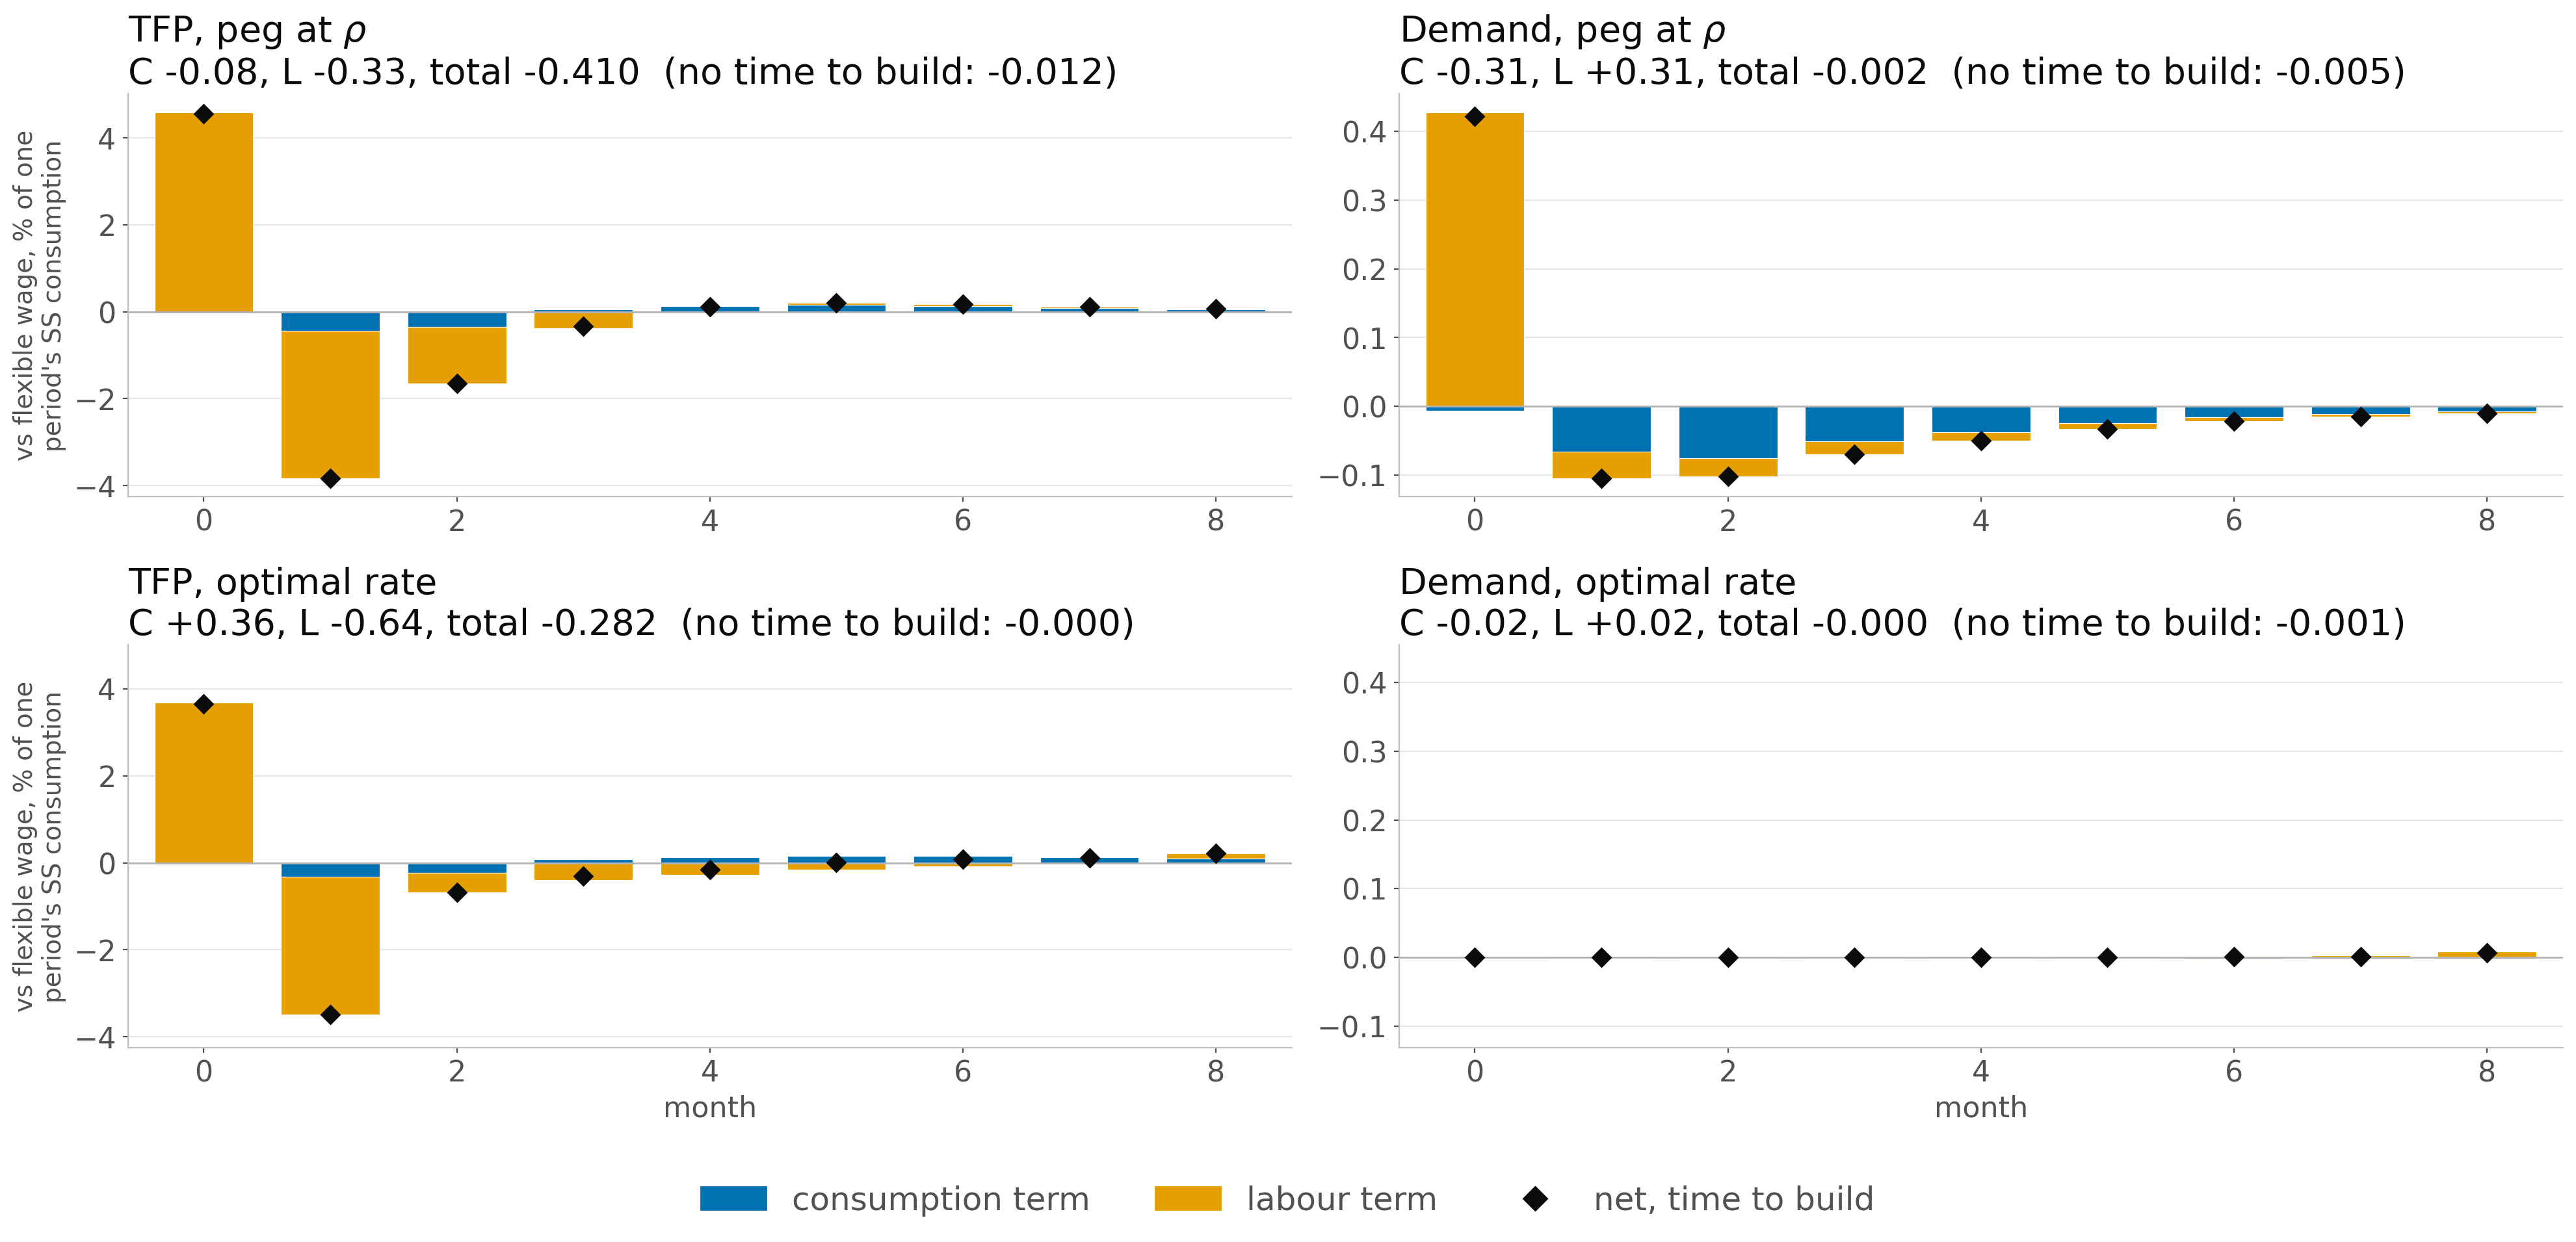
\includegraphics[width=\textwidth,height=0.76\textheight,keepaspectratio]{ttb_loss_unexpected.png}\end{center}
\end{frame}

\end{document}
